\documentclass{article}
\usepackage{tikz}
\usetikzlibrary{arrows.meta, bending}

\begin{document}

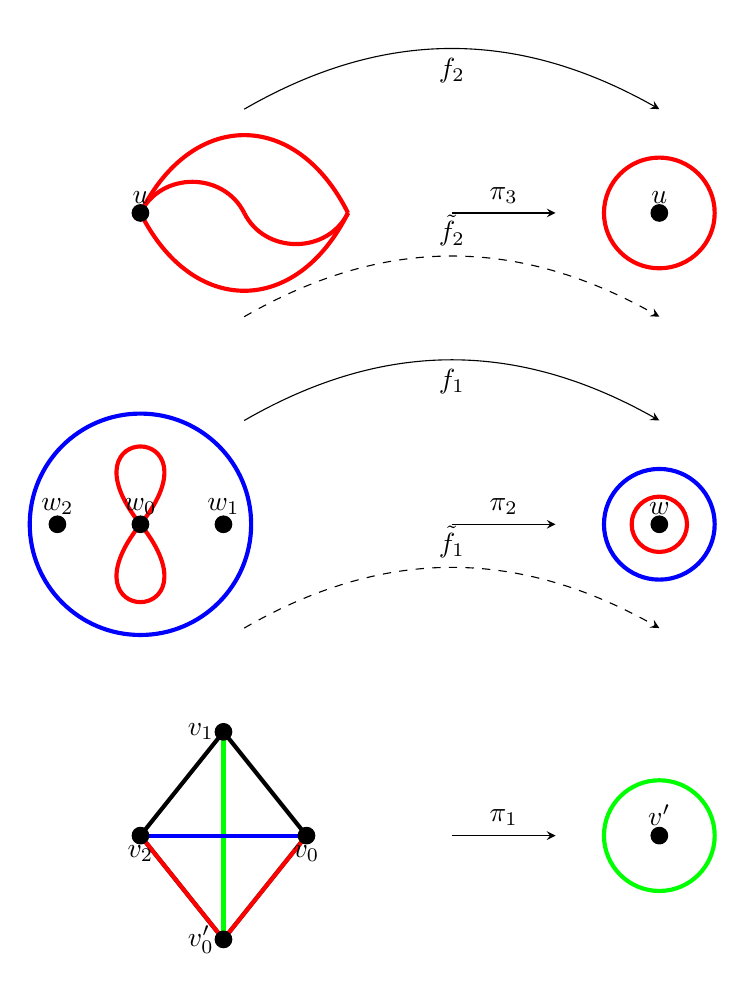
\begin{tikzpicture}[x=0.75pt, y=0.75pt, yscale=-1, xscale=1]

    % First Graph
    \draw[line width=1.5, red] (50, 100) .. controls (75, 50) and (125, 50) .. (150, 100);
    \draw[line width=1.5, red] (50, 100) .. controls (75, 150) and (125, 150) .. (150, 100);
    \draw[line width=1.5, red] (50, 100) .. controls (60, 80) and (90, 80) .. (100, 100);
    \draw[line width=1.5, red] (100, 100) .. controls (110, 120) and (140, 120) .. (150, 100);
    \draw[fill=black] (50,100) circle (3pt) node[above] {$u$};
    \draw[->, >=stealth] (200, 100) -- (250, 100) node[midway, above] {$\pi_3$};

    % Second Graph
    \draw[line width=1.5, red] (300, 100) circle (20pt);
    \draw[fill=black] (300, 100) circle (3pt) node[above] {$u$};

    % Morphism f2
    \draw[->, >=stealth, dashed, bend right] (100, 150) to node[midway, above, sloped] {$\tilde{f}_2$} (300, 150);
    \draw[->, >=stealth, bend right] (100, 50) to node[midway, below, sloped] {$f_2$} (300, 50);

    % Third Graph
    \draw[line width=1.5, blue] (50, 250) circle (40pt);
    \draw[line width=1.5, red] (50, 250) .. controls (10, 200) and (90, 200) .. (50, 250);
    \draw[line width=1.5, red] (50, 250) .. controls (10, 300) and (90, 300) .. (50, 250);
    \draw[fill=black] (50, 250) circle (3pt) node[above] {$w_0$};
    \draw[fill=black] (90, 250) circle (3pt) node[above] {$w_1$};
    \draw[fill=black] (10, 250) circle (3pt) node[above] {$w_2$};
    \draw[->, >=stealth] (200, 250) -- (250, 250) node[midway, above] {$\pi_2$};

    % Fourth Graph
    \draw[line width=1.5, blue] (300, 250) circle (20pt);
    \draw[line width=1.5, red] (300, 250) circle (10pt);
    \draw[fill=black] (300, 250) circle (3pt) node[above] {$w$};

    % Morphism f1
    \draw[->, >=stealth, dashed, bend right] (100, 300) to node[midway, above, sloped] {$\tilde{f}_1$} (300, 300);
    \draw[->, >=stealth, bend right] (100, 200) to node[midway, below, sloped] {$f_1$} (300, 200);

    % Fifth Graph
    \draw[line width=1.5] (50, 400) -- (90, 350) -- (130, 400) -- (90, 450) -- cycle;
    \draw[line width=1.5, green] (90, 350) -- (90, 450);
    \draw[line width=1.5, blue] (50, 400) -- (130, 400);
    \draw[line width=1.5, red] (50, 400) -- (90, 450);
    \draw[line width=1.5, red] (130, 400) -- (90, 450);
    \draw[fill=black] (50,400) circle (3pt) node[below] {$v_2$};
    \draw[fill=black] (90,350) circle (3pt) node[left] {$v_1$};
    \draw[fill=black] (130,400) circle (3pt) node[below] {$v_0$};
    \draw[fill=black] (90,450) circle (3pt) node[left] {$v_0'$};
    \draw[->, >=stealth] (200, 400) -- (250, 400) node[midway, above] {$\pi_1$};

    % Sixth Graph
    \draw[line width=1.5, green] (300, 400) circle (20pt);
    \draw[fill=black] (300, 400) circle (3pt) node[above] {$v'$};

\end{tikzpicture}

\end{document}